\documentclass[a4paper,onecolumn]{report}
\usepackage{caption}
\usepackage{subcaption}
\usepackage{setspace}
\usepackage{amssymb}
\usepackage[fleqn]{amsmath}
\usepackage{apacite}
\usepackage{graphicx}
\usepackage{color}
\usepackage{float}
\usepackage[toc,page]{appendix}
\usepackage[nottoc]{tocbibind}
\usepackage{titlesec}
\usepackage{float}
\usepackage{color}
\usepackage{setspace}
\usepackage{comment}
\usepackage{url}
\titleformat{\chapter}{\normalfont\huge}{\thechapter.}{15pt}{\huge}
\renewcommand*{\familydefault}{\sfdefault}
\hyphenpenalty=5000 
\tolerance=1000

\usepackage[a4paper]{geometry}
\voffset=-50pt
\hoffset=0pt
\topmargin = 0pt
\textwidth = 450pt
\textheight = 700pt
\marginparwidth = 10pt
\oddsidemargin = 5pt
\topmargin = 1pt
\graphicspath{ {/images/} }

\setcounter{tocdepth}{2}

\begin{document}

%----------------------------------------------------------------------------------------
%	TITLE SECTION
%----------------------------------------------------------------------------------------

\begin{titlepage}

\newgeometry{top=3in}

\newcommand{\HRule}{\rule{\linewidth}{0.5mm}}
\newcommand{\horrule}[1]{\rule{\linewidth}{#1}}

\center % Center everything on the page

\textsc{\small DELFT UNIVERSITY of TECHNOLOGY}\\[2.5cm] % Name of your university/college

\textsc{\LARGE Artificial Neural Networks}\\[0.5cm] % Major heading such as course name

\HRule \\[0.1cm]
\begin{spacing}{1.6}
{ \huge PROJECT REPORT}\\[-0.4cm] % Title of your document
\end{spacing}
\HRule \\[1.5cm]

\begin{minipage}{0.4\textwidth}
\begin{flushleft} \large
\emph{Authors:}\\
Michiel \textsc{Bongaerts} - 4096835\\
Marjolein \textsc{Nanninga} - 4096622\\
Tung \textsc{Phan} - 4004868\\
Maniek \textsc{Santokhi} - 4093968
\end{flushleft}

\end{minipage}
~
\begin{minipage}{0.4\textwidth}
\begin{flushright} \large
\end{flushright}
\end{minipage}\\[4cm]

{\large \today}\\[3cm]

\restoregeometry

\vfill

\end{titlepage}

%----------------------------------------------------------------------------------------
%	CONTENT
%----------------------------------------------------------------------------------------

{\small \tableofcontents}

\addtocontents{toc}{\protect\thispagestyle{empty}}

\chapter{Introduction}

Mapping the world around us has always been a human endeavor to advance economical output. A better understanding of the places around us makes for more efficient traveling and exploitation of the land. However, it has always been a very slow and tedious process to produce these maps, something technology has not changed just yet. A new opportunity has arisen with the arrival of satellite imagery and an ever increasing amount of computational power. An opportunity where this mapping can be done automatically so that this tedious and slow job can be processed even more quickly and perhaps more accurately. It is with this in mind we further analyze any possibilities.\\

The research question posed in this project, along with its clarification will be discussed in Chapter \ref{chap:researchquestion}. This is then followed by an elaboration on the conceptualization of the research question in Chapter \ref{chap:concept}, where we will discuss details of the system to be implemented, both chapters are written by taking into consideration the state-of-the art research.  The technical aspects of the system will be discussed in Chapter \ref{chap:softwarearchitecture}, detailing the inner workings of the framework which carries the neural network to be. The heart of our classification, the neural network, will then be elaborated upon in Chapter \ref{chap:CNN}, with the method of implementation of this network in Chapter \ref{chap:method}. Finally, the results and discussion will be described in detail in Chapter \ref{chap:resultsanddiscussion}.

\chapter{Research Question}
\label{chap:researchquestion}
One of the hardest aspects of image classification is the feature extraction. Traditionally this was done by a seperate feature extraction \cite{duda1973pattern}, which was necessary mainly because no computers were available that could process the high-complex algorithms and because large datasets to train and test could not be found yet \cite{lecun1998gradient}. However, this manual choice is of feature extraction is suboptimal, since it is empirical and bad choices can strongly influence the results \cite{duffner2008face}. 
Another possibility is to fully connect all the raw pixels from the input image to a Multilayer Perceptron (MLP) and use backpropagation to find the feature extractors. Because of the extremely high input dimension of pictures, the number of free parameters is also extremely large and an infinite number of training data should be used to avoid overfitting \cite{hawkins2004problem}. \\

In initial research we found a new solution into image classification problems and in particular satellite image classification: the Convolutional Neural Networks (CNN) \cite{Hongsheng2014} \cite{Farabet2013}. The literature is showing that using Convolutional Neural Networks (CNN) would introduce interesting properties to base our research and subsequent project implementation on (see Chapter \ref{chap:CNN}).\\

The process of feature extraction is incorporated in the training of Neural Network. The backpropagation, which is part of these CNNs, facilitates that all the weights of the layers are adjusted iteratively, and therefore it eliminates the need to manually create the convolution masks with which the features are being extracted. Another advantage of using CNN is the ability to take into account correlations of neighboring input data, which are plentiful in satellite images. Convolutional Neural Networks also make use of the principle of weight sharing in convolutional layers, which further reduces the amount of free parameters. In literature it is indeed shown that the CNN automatically learns local feature extractors, they are invariant to small translations and distortionts, but due to the pooling layers drastically reduce the input dimension \cite{duffner2008face}.

Given these properties, it is understandable that most of the papers we encountered within the context of our problem make use of Convolutional Neural Networks.\\

We described that extracting features manually can lead to suboptimal results. However, suboptimal outcomes could also be the result of the large amount of variations possible in CNNs within the given context. It is therefore interesting to explore this optimality dimension with the following research question:

\begin{quote}
\emph{ \hspace{2ex} For satellite image classification to identify forest, water and city, what is the best Convolutional Neural Network configuration that exploits the feature extraction generality of CNNs?}
\end{quote}

This research is about constructing a CNN that can classify satellite imagery well for the labels: forest, water and city while retaining the notion to not specifically extract features manually. Empirically the answer to this question will be researched in which the appropriate boundaries will be set to come to a conclusion in an effective manner. Also a competing notion to the feature extraction generality of CNNs will be explored as a discussion mean.

\chapter{Concept}
\label{chap:concept}
Earlier attempts to conceptualize the idea to automate map making resulted in a proposal that too heavily focused on the actual map creation rather than the classification. For a Neural Network course this was deemed not befitting enough. The plan was also quite far reaching to start with. Thoughts were put into downscaling this ambitious plan. We played around a bit and came up with a new concept which will be discussed in this chapter.\\

Firstly, an impression is given how the end user interacts with our system. This will lay the groundwork for how the Neural Network will be constructed. Actual talk about the classification is done in the subsequent chapter. Secondly, through the principles of MoSCoW, a flexible requirements list is established. An evaluation of said requirements is lastly provided. 

\section{Impression}

Below in Figure \ref{fig:impression} an impression is given of what the end user will interact with and a possible result that might come about from said interaction.\\

\begin{figure}[h!]
    \centering
    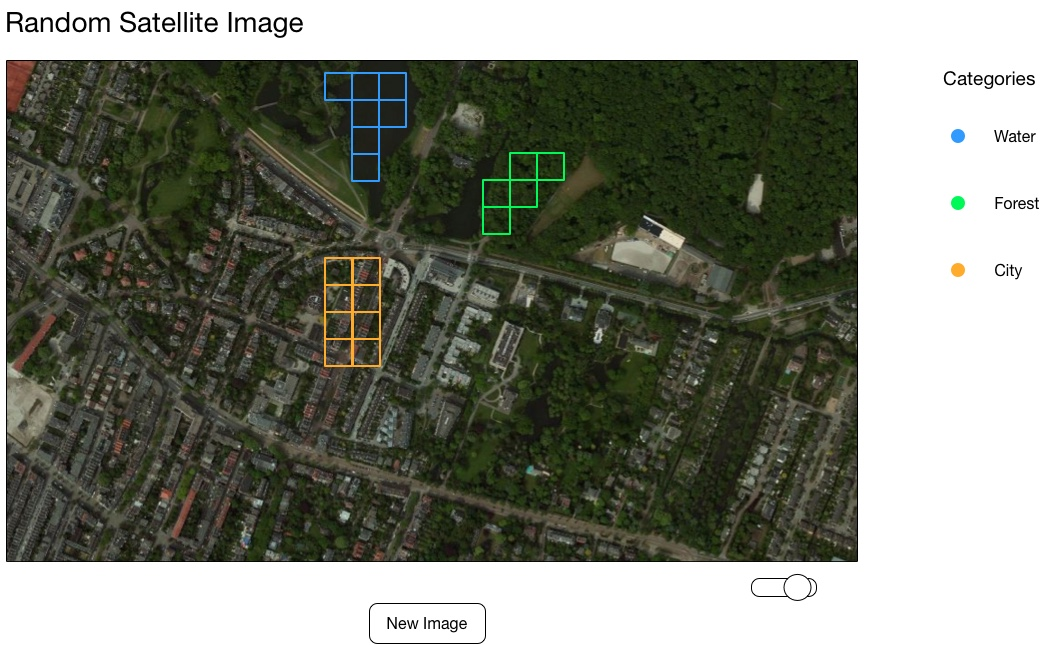
\includegraphics[width=0.8\textwidth]{./images/impression_toggle.jpg}
    \caption{Impression of what the user interacts with and a possible outcome.}
	\label{fig:impression}
\end{figure}

The most notable attention grabber is the satellite image. This image will be acquired through a random call from a homogeneous satellite image database on every new instantiation of the system. Another possibility to acquire new data is by clicking on the 'New image' button. Right of the satellite image one can see labels (Forest, City, Water) which correspond with the labels which are outputs of the classification. Results obtained from our algorithm, given the current satellite image as input, are graphically fed back to the user. The impression above does that by showing a correspondence between image patches (squares) and their respective label via color coding laid over the satellite image. This rendition just shows a few islands of results as an example. Normally the entire image will have such arching.\\

In order to classify the satellite image, the map is first divided into patches of predetermined dimensions. These patches are squares, the dimensions should be divisible by $2$ (as will be explained later) and these are the main, large patches to be fed into the neural network to be classified. The network will label the patches and return the outcome. The outcome is then evaluated to be rendered like is shown in Figure \ref{fig:impression}.\\

However, we wanted to give the user the choice of making a more detailed classification with a smaller grid size without altering the workings of the neural network. To do so, an additional grid overlay is created with a small modification to the original rendering algorithm: the large patches now overlap each other in both dimensions by a half (hence that the large patches should be divisible by $2$). So if the map can be divided into N large patches in the width and M large patches in the height, this new setup will now have $(2N - 1)$ patches in the width and $(2M - 1)$ patches in the height, discarding patches that are halfway out of bounds. These patches are then fed to the neural network in the exact same fashion as the previous method. A second grid overlay is then effectively created, with the size of these smaller patches exactly a quarter of the larger patches. 
Figure \ref{fig:grid} provides a visual aid of this process, with the green patch indicating the large patch and the red patch indicating the resulting smaller patch.\\

The idea is to link these smaller patches to its four larger patches, as these are its labeled parents. The labels of the parents were determined by the network by giving it a certainty between 0 and 1 for each class, with 1 the highest certainty this patch belonged to the corresponding class.
A weighted majority vote is then used by summing the values of these classification of each of the four parents, grouped by their classes. The highest sum will be picked as the winner of the majority vote and its corresponding class will be used as a label for the smaller patch.\\

For example, if there are three possible classes, $A$,$B$ and $C$, the certainty values of a patch can be denoted as $\{a_i, b_i, c_i\}$ where $1 \leq i \leq 4$. The values of the four parents of a small patch are then weighted, so you end up with $\{ \frac{1}{4}\sum_{i=1}^{4} a_i, \frac{1}{4}\sum_{i=1}^{4} b_i, \frac{1}{4}\sum_{i=1}^{4} c_i\}$. Whomever is biggest, wins. Doing this for all $(2N - 1) \times (2M - 1)$ patches results in a new classification grid showing more detail. This in turn allows the user to make a finer classification and switch back and forth accordingly via the toggle button displayed in the impression of Figure \ref{fig:impression}.

\begin{figure}[h!]
    \centering
    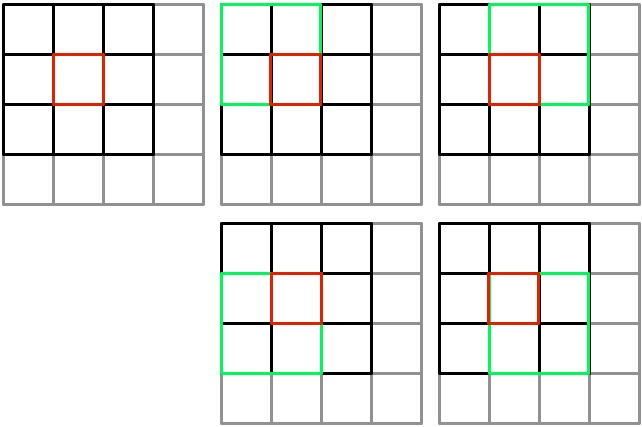
\includegraphics[scale=0.6]{./images/grid_explained.jpg}
    \caption{Grid structure which facilitates the algorithm, green denotes a large patch, while red denotes the small patch. Here is illustrated how the red, smaller patch has four green, larger parent patches.}
	\label{fig:grid}
\end{figure}

\section{MoSCoW}
\label{sec:MoSCoW requirements}
Since our time to work on this project is limited while the amount of goals we wanted to accomplish in this period were numerous, we used the MoSCoW analysis technique to prioritize these goals and focus on the most important requirements. MoSCow stands for \textit{Must have}, \textit{Should have}, \textit{Could have} and \textit{Would have}, with the importance of each category ordered in a descending fashion. This enables us to identify core requirements which are absolutely necessary for the functionality of our implementation and in turn enables us to set up the core functionality first before focusing on the secondary objectives. All the requirements are labeled in these four classes. These requirements were laid out before the concept we eventually pursued had taken shape.\\

\subsection{Must have}
Must have requirements are critical to project success. 
\begin{itemize}
\item Implement a working \textit{Convolutional Neural Network} (CNN) that enables automatic classification of patches from satellite images. Considering images acquired on provincial level and a substantial amount of pixels in one patch (at least 50 x 50 pixels). 
\item At least the following classes should be recognized: vegetation, city and water. 
\item Develop a way to visualize the automatic classifications clearly.
\end{itemize}

\subsection{Should have}
Requirements labeled as `Should have' are important to book success, but not necessary for delivery.

\begin{itemize}
\item Create a clear interface in which the unlabeled images can be uploaded, and the output consists of labeled images. 
\item Calculate the uncertainty in the classification and ask user input for very uncertain patches.
\end{itemize}

\subsection{Could have}
It would be very nice if we would be able to reach the Could have features, but they are not critical. 
\begin{itemize}
\item Experiment with preprocessed images (noise reduction, gradient calculations)
\item Analyze images on city level, so with more details present. For this purpose new classes have to be added, such as roadways, cycle paths, 	buildings, distinct vegetations etcetera. 
\item Experiment with other models than the state-of-the art \textit{LeNet-1 CNN}. For examples, a CNN in which \textit{Genetic Algorithms} are incorporated, or implementing an \textit{Extreme Learning Machine} for the training of the weights. 
\end{itemize}

\subsection{Would have}
These requirements are implemented only in the most ideal situation. They are considered as the dream project, sometimes serving as a suggestion for further projects. 

\begin{itemize}
\item Develop a method for high-detailed automatic vector graphics, in which segmentation of the distinct labeled classes is incorporated.
\item Use the input of the users to improve the automatic classification. 
\item Sell the software package to Google. 
\end{itemize}

The evaluation of these requirements can be found in the Results in Section \ref{sec:Evaluation MOSCOW}

\chapter{System design}
\label{chap:softwarearchitecture}
A plan has been established what kind of application should come about. The previous discussion pressed for a certain kind of structure. One where a Neural Network is central to the problem to be solved. But also a front end is needed for certain user interaction as well as an infrastructure in the back end which facilitates the communication with said front end. This chapter discusses the infrastructure setup, the technologies used and the data being acquired.

\section{Infrastructure}
The impression given above in Figure \ref{fig:impression} is close to what the end result of the implementation will look like (although it only displays a certain state). Yet an entire infrastructure outside of the Neural Network is needed to facilitate the application. Below in Figure \ref{fig:communication} an infrastructure is visualized via the communication of the two entities.

\begin{figure}[h!]
    \centering
    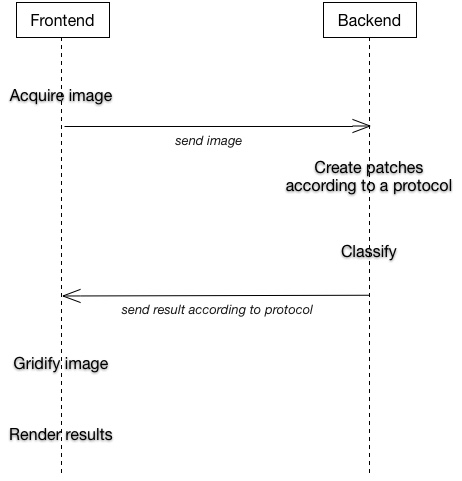
\includegraphics[scale=0.5]{./images/communication2.jpg}
    \caption{Communication visualization between front end and back end.}
	\label{fig:communication}
\end{figure}

First, at the front end, an image is acquired by the user from a map API call. The image is immediately sent to the back end. There, patches are extracted according to a certain protocol (specific size and sequence) which also depend on whether small or large patches need to be visualized. The patches are classified by our Neural Network. Send back to the front end are the label results in a list according to the sequence defined by the protocol mentioned earlier. Back at the front end the image is made into a grid which also corresponds to the size and sequence of the protocol. The squares in the grid are then colored in according to the labels in the list that had been sent back.

\section{Technical Details}
The front end consists of a web based interface, capable of visualizing the map acquired with the Bing Maps API \cite{bing}, the controls enabling the user to interact with the system and the resulting classification. The web application runs on Node.js and ZeroRPC. Node.js is an event-driven I/O server-side JavaScript environment and ZeroRPC is a cross-language RPC library, capable of performing remote procedure calls. Using these calls, we can effectively communicate with the Neural Network, written in Python, which is hosted on another server. The idea of this setup was to make it scalable: the initial plan was to implement the Neural Network with the idea of on-line learning, meaning the network could use a considerable amount of resources while running. If this network was hosted on the same server as the web server, this could be detrimental to the performance of both services.

\section{Map dataset}
The satellite imagery used in this project is acquired from the Bing Maps database \cite{bing}. A predefined size of the map is displayed on the front end, with satellite view enabled at a height of 100 meters. The labels were turned off, along with other controls or visible logos, which could interfere with the classification.  A random location inside the Amsterdam area is generated.\\

For training, satellite images from the same source and practice mentioned above are drawn on a per category/label basis. Meaning: specific images of locations only showing one category (water, forest, city) are being taken. Then patches are acquired code-wise over those images so that for each patch it is known what category/label belongs to it. Every patch has a size of 40x40 pixels. These images are taken from a larger corpus than the Amsterdam area, from across the world but focussing on the Netherlands. This way of acquiring labelled data was done for efficiency purposes, but is suboptimal; an entire image is classified in one class, when in reality they contain patches from the other classes. For example, all cities have some park, gardens and pools. When the larger image is divided into smaller patches, patches containing just gardens labeled as city appear. Moreover, because an image is saved as a rectangle, the patches from the outer edge of the cities, water and vegeation are left out (since otherwise they would contain other classes as well). However, water for example has another structure and colour close to the water edge, and these patches are not included in the training data. 

\chapter{Convolutional Neural Network}
\label{chap:CNN}
A typical CNN architecture consists of multiple convolution layers and sub-sampling layers. It depends on the architecture in what sequence these layers occur. The convolution layer is the resulting layer after the convolution operator is performed by the convolution kernel. Since the goal is to extract general features from our input image, we want the CNN to generalize. This generalization is partly realised by dimension reduction. Since convolution operations reduce the dimension of our input map with $\frac{M-N+1}{M}$, where $N$ is the dimension of the convolution kernel and $M$ the dimension of the input map, we want the dimension to be reduced more quickly. This is done by sub-sampling kernels which basically 'squeeze' or average the input map with a certain dimension. This operation is equivalent to a convolution operation but with a larger step-size (convolution uses a step size equal to 1) and equal weights for each element in the sub-sampling kernel.

\section{LeNet-1}
The model we implement is LeCun's LeNet-1 \cite{lenet}. This model uses an alternating sequence of convolution and sub-sampling or pooling layers. The architecture of this network is shown in Figure \ref{fig:Architecture}. The convolution layers act as feature maps, they consist of a window of a certain size, whose pixels are trainable weights. The sub-sampling layers reduce the dimensionality of the outputs. 
\begin{figure}[h!]
    \centering
    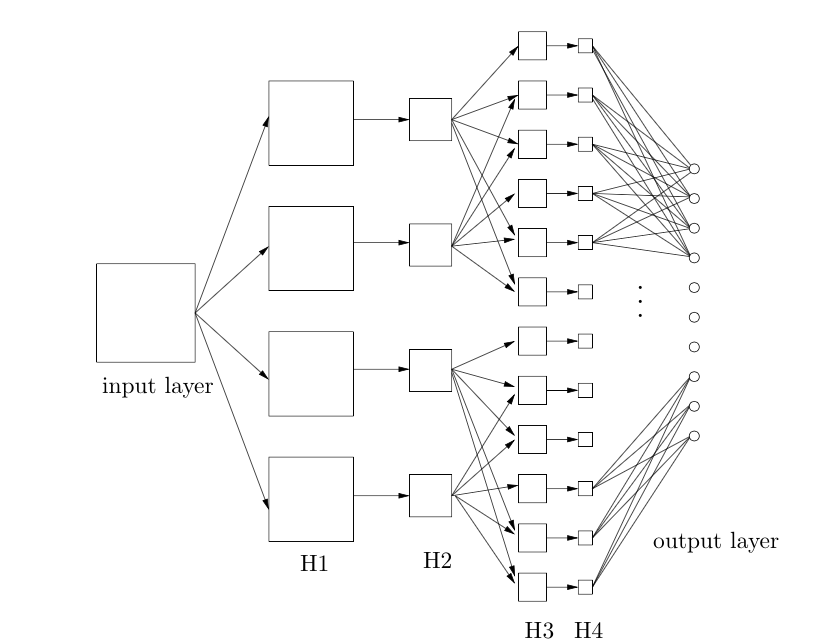
\includegraphics[scale=0.4]{./images/Architecture_CNN.png}
    \caption{The architecture of the CNN proposed by LeNet. H1 and H3 are the convolution layers, H2 and H4 the sub-sampling layers to reduce the dimension. }
	\label{fig:Architecture}
\end{figure}

One of the biggest advantages of using CNN, and especially LeCun's LeNet-1 implementation, is the incorporation of backpropagation learning. Meaning that all the weights of the layers are adjusted iteratively, eliminating the need to manually create the convolution masks.\\

The final architecture we used for the application will be discussed in Section \ref{sec:finalimpl}

\section{Backpropagation}
\label{sec:BP}
To train the network, we have to adjust several parameters in the network. In this research we consider backpropagation from the output layer to layers H4 and H3. In the whole network we use the Sigmoidal activation functions, defined as:
\begin{equation}
f(x)=\frac{1}{1+e^{-x}} 
\end{equation}	
The error function is defined as:
\begin{equation}
E=\sum_{k} \frac{1}{2}|t_k-F_{k}|^{2}
\end{equation}
Where $t_k$ represents the labeled class of the training and $F_{k}$ is the corresponding activation of the classifier neuron . This variable is 1 if the corresponding class is trained and 0 if this is not the case. \\

Below the functions are listed in which we go from the activation of our classifier neuron to weights present in layer H3. In these equations $r$ stands for row which is the first branch after the first convolution i.e. the total rows is equal to the amount of different feature maps in H1. $b$ stands for the amount of branches per row. $k$ stands for the amount of classes which are trained by the network.
\begin{equation}
\begin{split}
	&F_{k}= f( x_{k}) \\
	& x_{k}=\sum_{ij} W^{4rbk}[i,j] \; H^{4rb}[i,j] - b_{k} \\
	&H^{4rb}[i,j]= \sum_{u,v} W^{3rb}[u,v] \; H^{3rb} [2i+u,2j+v] \\
	&H^{3rb} [2i+u,2j+v]= f\left (x^{3rb}[2i+u,2j+v] \right) \\
	&x^{3rb}[2i+u,2j+v]=\sum_{nm} W^{2rb}[n,m] \; H^{2rb}[n+(2i+u),m+(2j+v)] -b^{3rb}
\end{split}
\end{equation}
In the above equations $i$ and $j$ are the row and column respectively for the elements in the output maps and end-weight matrix $ W^{4rbk}$. The superscript in the latter indicates for layer H4 and corresponding row $r$ and branch $b$. The elements $u$ and $v$ are the elements over the sub-sampling kernel where $n$ and $m$ are the elements over convolution kernel $W^{2rb}$.\\

From these equations we can calculate the update-rules for backpropagation. This is done by applying the gradient descent method in which we calculate the derivatives of the error function. The update-rule consists of the derivative with respect to the parameter we want to update. For updating $W^{4rbk}$, also called the end-weights, we use:
\begin{equation}
\begin{split}
\Delta W^{4rbk}[i,j]&= \sum_{k} - \eta \frac{dE}{d F_{k}} \frac{dF_{k}}{dx_{k}} \frac{dx_{k}}{dW^{4rbk}[i,j]} \\
&= \sum_{k} \eta (t_{k}-F_{k})\frac{e^{-x_{k}}}{(1+e^{-x_{k}})^{2}} \frac{dx_{k}}{dW^{4rbk}[i,j]} \\
&= \eta (t_{k}-F_{k})\frac{e^{-x_{k}}}{(1+e^{-x_{k}})^{2}} H^{4rb}[i,j]
\end{split}
\end{equation}
For updating the bias $b_{k}$ corresponding to each classifier neuron:
\begin{equation}
\begin{split}
\Delta b_{k}= - \eta \frac{dE}{d F_{k}} \frac{dF_{k}}{dx_{k}} \frac{dx_{k}}{b_{k}}=\eta (t_{k}-F_{k})\frac{e^{-x_{k}}}{(1+e^{-x_{k}})^{2}} (-1)
\end{split}
\end{equation}
The updating for the elements in the convolution kernel $ W^{2rb}$ requires some more derivatives:
\begin{small}
\begin{equation}
\begin{split}
	&\Delta W^{2rb}[n,m] = \\
	&\sum_{k} - \eta  \frac{dE}{dF_{k}} 
	\frac{dF_{k}}{dx_{k}} 
	\sum_{ij} \frac{dx_{k}}{dH^{4rb}[i,j]} 
	\sum_{uv}\frac{dH^{4rb}[i,j]}{d H^{3rb} [2i+u,2j+v]} 
	\frac{d H^{3rb} [2i+u,2j+v]}{d x^{3rb}[2i+u,2j+v]}
	\sum_{nm}\frac{d x^{3rb}[2i+u,2j+v]}{d W^{2rb}[n,m]} \\
	=&\sum_{k} \sum_{ij} \sum_{uv} \sum_{nm}  \eta (t_{k}-F_{k})\frac{e^{-x_{k}}}{(1+e^{-x_{k}})^{2}} W^{4rbk}[i,j]  W^{3rb}[u,v] \frac{e^{-x^{3rb}[2i+u,2j+v]}}{(1+e^{-x^{3rb}[2i+u,2j+v]})^2} \\
	 & H^{2rb} [n+(2i+u),m+(2j+v)]
\end{split}
\end{equation}
\end{small}
Since there is also a bias $b^{3rb}$ present in layer H3 we have to update these weights as well:
\begin{small}
\begin{equation}
\begin{split}
	&\Delta b^{3rb} =\\
	&\sum_{k} - \eta  \frac{dE}{dF_{k}} 
	\frac{dF_{k}}{dx_{k}} 
	\sum_{ij} \frac{dx_{k}}{dy^{4rb}[i,j]} 
	\sum_{uv}\frac{dy^{4rb}[i,j]}{d y^{3rb} [2i+u,2j+v]} 
	\frac{d y^{3rb} [2i+u,2j+v]}{d x^{3rb}[2i+u,2j+v]}
	\frac{d x^{3rb}[2i+u,2j+v]}{d b^{3rb}} \\
	&=\sum_{k} \sum_{ij} \sum_{uv} \eta (t_{k}-F_{k})\frac{e^{-x_{k}}}{(1+e^{-x_{k}})^{2}} W^{4rbk}[i,j]  W^{3rb}[u,v] \frac{e^{-x^{3rb}[2i+u,2j+v]}}{(1+e^{-x^{3rb}[2i+u,2j+v]})^2} (-1)
\end{split}
\end{equation}
\end{small}
\begin{small}
\begin{equation}
\end{equation}
\end{small}


\chapter{Method}
\label{chap:method}
In developing the final architecture, choosing the type of training patches, the number of classes and the amount of training data, well considered decisions had to be taken where to put the focus: more on the application itself or on the research. E.g. when taking only water patches from the middle of the ocean where the colour and structure is very similar, it is very easy to achieve a high accuracy in the research phase. However, these patches are not similar at all to the the somewhat filthy canals of Amsterdam, so the performance of the application will be poor. In the end, we focussed on a system that has a good application performance, implying a lot of variance within the distinct classes and we experimented with both 3 and 4 classes in the application itself. 

\section{Variables within architecture}
The architectures of the Convolutional Neural Networks we use for this research are based on the LeNet-1 described in chapter \ref{chap:CNN}. The architectures could differ in several ways from each other. First, we can adjust the sizes and types of the first convolution kernels. Second, the dimension reduction for both sub-sampling kernels can differ. The size of the second convolution kernels can be changed and the dimension of the output map (H4) can be chosen differently. At last, the amount of classifier neurons at the end of the network can be modified but this necessarily depends on the amount of classes the network has to resolve. 

\section{RGB values}
\label{sec:RGB}
The literature we found primarily focuses on hand-written document recognition and facial recognition, both assuming grey-scale images. The images available to us are colour images, so a decision had to be made about what information to take into account. To train the system on the structure using the architecture above we used the so-called relative luminence $Y$, reflecting the human visual perception: green light contributes most to the intensity perceived by humans and blue light the least \cite{stokes1996standard}:
\begin{equation}
Y=0.2126 R+0.7152 G+0.0722 B
\end{equation}
\noindent
In which R, G, and B indicate the red, green and blue RGB value respectively.\\

Because it was assumed that the colour itself could provide information on the class it should be classified in, we experimented with taking this information into account as well. That was done by calculating the average intensity of the R, G and B values of every patch and adding 3 nodes to the output nodes. The normalized average intensity of the patches was fed as an input to these 3 nodes and the corresponding weights were trained in the same way as the other output nodes. This eventually would serve us as the competing notion to our research question, where we investigate the feature extraction generality of Convolutional Neural Networks. 

\section{Final architecture implemented in application}
\label{sec:finalimpl}
To investigate which architectures are sufficient to use for our application a few architectures were explored. The various parameters as described above are changed resulting in different network designs. We focussed on a system that automatically learns the feature extraction, but we were limited in the complexity of the architecture because of the time available and because we did not have acces to large GPU's and GUI's. That is why we developed a relatively small architecture in which only the first convolution layer was predefined. The following components in our architecture were used:

\begin{itemize}
\item \textbf{Input layer}: consisting of 40x40 pixels from satellary images, combining the R,G and B values as mentioned in Section \ref{sec:RGB}.
\item \textbf{First Convolution layer}: Consisting of two kernels of 9x9 pixels. For these kernels we chose one Kernel inspired on the Sobel operator in the X-direction and the other in the Y-direction. We chose these 2 kernels since the Kernels are X and Y edge-detectors and we considered this as the most logical first feature extractors \cite{kanopoulos1988design}. Using these kernels results in a H1 layer of two images of size 32x32 pixels.
\item \textbf{First sub-sampling layer} Consisting of a 4x4 pixel kernel all with the same weight. The use of this kernel is two-folded: dimension reduction and normalization of the data (data divided by 1/100). This layer results in a H2 layer of 2 images of 8x8 pixels
\item \textbf{Second Convolution layer}: This is the layer that is used for the automatic feature extraction. Per row (two rows are considered) 3 kernels are used. Every Kernel has a size of 5x5 pixels. The weights of the Kernel are assigned according to a random uniform distribution on [0,1]. This architecture results in a H3 layer of 2x3 images all consisting of 4x4 pixels.
\item \textbf{Second sub-sampling layer}: this layer is just used to normalize the data again. So it consists of just one pixel of weight 1/10. 
\item \textbf{Final layer}: consists of all the pixels from layer H4, and in case the RGB colours are considered as well, 3 nodes are added with the average intensity as input. This final layer is fully connected to the output layer. 
\item \textbf{Output} We consider for this research section a three-class system: Forest, City and Water. So the output consists of 3 nodes.
\end{itemize} 

The network can be trained in two different ways: backpropagation on the classifier neuron biases ($b_{k}$) and end-weight ($ W^{4rb}$) or the latter and a further backpropagation process where also the weights of the second convolutional kernels are trained ($ W^{2rb} $) together with their biases ($b^{3rb}$). We started with investigating how the networks perform when we only do the first type of training since further backpropagation will be more computationally expensive. Their performance is measured with a method based on cross-validation.\\

In the end we used the afore-mentioned architecture and we tested the performance of the following settings: 
\begin{itemize}
\item Taking no colours into account, and backpropagation limited to the end-weights.
\item Taking the colours into account, and backpropagation limited to the end-weights.
\item Taking no colours into account, and backpropagation until the second convolution layer.
\item Taking the colours into account, and backpropagation until the second convolution layer. 
\end{itemize}


\subsection{learning rates}
The performance of the architecture was highly dependent on the learning rates used. When initializing large learning rates can be chosen so that the network learns roughly how to recognize the classes, but moving further only detailed information can be withdrawn by adjusting the learning rates. We heuristically experimented a lot with the learning rates and in the end came up with a system in which the learning rates were lowered by approximately a factor of 5 after 5000 samples. 

\subsection{Cross Validation}

To compare the different architectures we used a cross-validation based method. This includes the training of the network on 90\% of the data/total amount of patches. The remaining (revolving) 10\% is used to validate the performance of the network. In the test phase the values are calculated by the relative fraction of correctly assigned patched, or: 

\begin{equation}
\label{eq:P}
P= \frac{N_{right}}{N_{right}+ N_{wrong}}
\end{equation}

The final value is chosen by averaging over the 10 test sets, and the uncertainty is defined as the standard deviation within these test sets.\\

The total amount of patches used was 21407, of which 7163 forest patches, 6350 city patches and 7894 water patches. 

\section{Programs and packages to develop the CNN}
The networks were programmed in \textit{Python}. No special packages related to Neural Networks were used such as \textit{Theano}.  So we completely built the architecture ourselves. For the convolution operation, we used the package \textit{Scipy.signals} which contains a convolution function. Furthermore, some additional packages were used for basic operations in the program such as \textit{Numpy} and \textit{PIL}. The latter is used to import images for the root. Since we use patches to train the network, we write a function which divides the imported images in patches. Each patch gets the label corresponding to the class it belongs to so it can be used to train the network. The images were obtained from Bing Maps \cite{bing}. Suitable images were gathered by selecting only places which contains the favored class. An example is shown in Figure \ref{fig:classexample}. A side note has to be included for the images with the class city since these images may include some tree, grassland or water patches and thus will be labeled with the class city. Most other classes, such as forest, grassland and water, does not entail this problem since a great proportion of the world contains purely these classes.

\begin{figure}[h!]
    \centering
    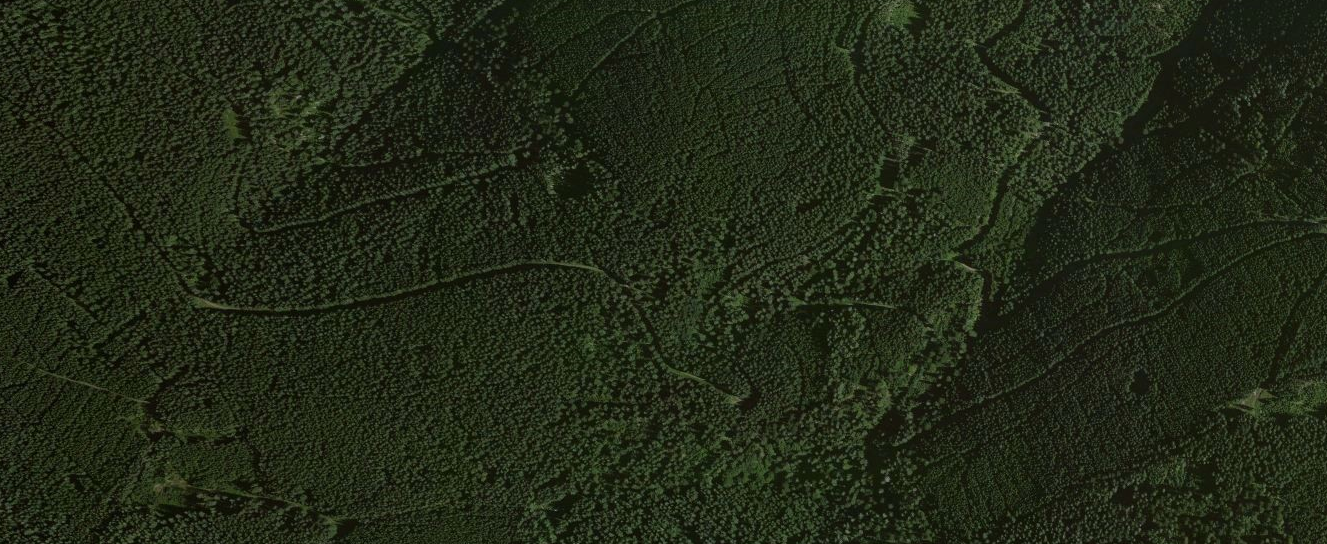
\includegraphics[scale=0.4]{./images/classexample.png}
    \caption{Example of a training image for the forest class.}
	\label{fig:classexample}
\end{figure}



\chapter{Results and Discussion}
\label{chap:resultsanddiscussion}
Now that the implementation has been finished, first of all an overall evaluation of the system will be given by evaluation whether the initial MoSCoW requirements were met, see Section \ref{sec:MoSCoW requirements}. Subsequently, an elaboration on the results regarding the research on the different architectures will be given. 


\section{Evaluation of the MoSCoW requirements}
\label{sec:Evaluation MOSCOW}


\textbf{Must have}\\
As the name of the Must have category implies, these requirements are critical to the success of the project and as such, these requirements were all met. The CNN is designed and is trained beforehand, the resulting weights are then injected into the CNN placed on the server, used to classify the map patches. The CNN is capable of distinguishing three separate classes, with an experimental CNN capable of distinguishing four classes (further elaborated on in Section \ref{chap:resultsanddiscussion}).
A basic web interface was created, with the ability to highlight specific classes to help visualize the classification of the network. It should be noted that the 50x50 pixel patches were not set in stone, but it was a good general guideline (we eventually settled for patches of 40x40).\\
\\
\textbf{Should have}\\
Due to time constraints, some requirements had to be modified in order to implement them or were left out altogether. The ability to upload own satellite imagery was replaced with the ability to acquire random satellite imagery of Amsterdam and its surroundings, which are in turn classified by the network. Choosing this route means that we can worry less about content validity and security of the application. The calculation of uncertainty is possible, but the implementation of user correction in conjunction with this uncertainty was left out. This is due to time constraints and the fact that we have not implemented on-line learning, but rather let the network train off-line beforehand, making this feature obsolete.\\
\\
\textbf{Could have}\\
Preprocessing the images might have had a positive influence on the classification results. However, the goal of this project was to implement a Neural Network that could learn on its own what the best discriminating features of a satellite image is, given the context. The option to classify maps on different altitude levels is not implemented, also due to time constraints. Different levels of altitude means to either have a general neural network that works on all altitudes, or having to train the network on different altitudes in order to produce multiple weight setups. Both of these options meant more time needed to develop, implement and test the new setups. We did manage to implement a good general neural network, but we did not have time to test this functionality properly on different altitudes. However, different setups have been experimented with, which will be discussed in Section \ref{chap:resultsanddiscussion}.\\
\\
\textbf{Would have}\\
The would haves requirements were on a whole different level and thus are self-explanatory why they weren't implemented.

\section{Quantitative results}
The quantitative results consists of different parts. First, to choose the different architectures that we wanted to research into detail we needed an overall idea of what works good and what does not. To do this we built a lot of different architectures, manually setting kernels and in this way empirically testing different architectures. The general results are mentioned first. Subsequently, an elaboration of the detailed results of the cross validation is included. Finally, we tested some more complex architectures to research its potentional in future research. These results are included in Appendix \label{app:DiffentArchitectures}.

\subsection{Results of manually selecting kernels}
In the first phase of our research we made a convolutional neural network based on LeNet-1. We experimented with different convolution kernels in the first layer (H1) of the network and differed the amount of branches in the third layer (H3). We started with manual empirically chosen convolution kernels for both layers H1 and H3. We began with input patches of 50 x 50 followed by a convolution kernel of 5x5 resulting in a feature map of dimensions 46x46. Next, sub-sampling with a dimension reduction of 2 results in a feature map of dimension 23x23. Again we did different 4x4 convolution kernel operation creating branches in H3 resulting in 20x20 feature maps. Sub-sampling with a dimension reduction of 5 resulted in an 4x4 output map. These output maps are then connected to two different classification neurons for Forest and City. \\

We used the Sigmoid function as activation function only for our classification-neurons. Thus, no activation functions were used earlier in the network (compared to LeNet-1). We performed backpropagation on the weights connecting the output maps with the classification neurons and biases. The first functioning results where found with 4 feature maps in H1 and 2 feature maps in H3 each where the network was enabled to recognize some forest/city patches from an new image. These results were too poor to include in this report. We used the convolution kernels shown in figure \ref{fig:firstFilters}. The Network was trained on structure only so no color features were included. 
\begin{figure}[h!]
	\centering
	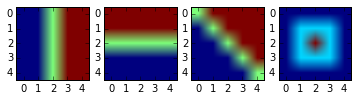
\includegraphics[width=0.5\textwidth]{./images/firstFilters.png}
	\caption{The four filters used in the first stage where the CNN was able to distinguish forest and city.}
	\label{fig:firstFilters}
\end{figure} 

In the second phase we tried to extend our classes with the class \textit{water} or \textit{grassland}. From the first few runs it turned out that the networks found it hard to distinguish the classes \textit{forest} and \textit{water}. By comparing some patches of both classes it became quite evident that this distinction is hard since their structure is similar (see Figure \ref{fig:WaterForestPatch} ). For this reason we included the class \textit{grassland} instead of \textit{water}. From figure \ref{fig:GrassForestPatch} we can see that these patches are less similar and thus we would expect the network to perform better on this combination of classes.

\begin{figure}[bth]
	\centering
	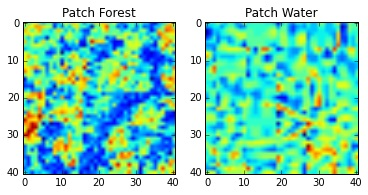
\includegraphics[width=0.5\textwidth]{./images/WaterForestPatch.jpg}
	\caption{A forest and water patch are shown. Their similarity makes it hard for the CNN to distinguish these two classes.}
	\label{fig:WaterForestPatch}
\end{figure}
\begin{figure}[bth]
	\centering
	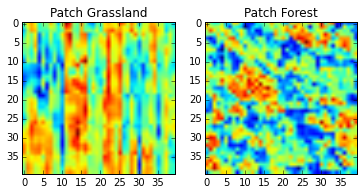
\includegraphics[width=0.5\textwidth] {./images/GrassForestPatch.jpg}
	\caption{A grassland and forest patch are shown.}
	\label{fig:GrassForestPatch}
\end{figure}


During this phase we tried to investigate whether training only the end-weights ($W^{4rb}$) and biases ($b_{k}$) were sufficient to train the network to classify three classes. We experimented with different types of architectures for the networks. We trained nine networks with different sub-sampling operations. Also the sizes of the convolution kernels and the dimension of the output maps were varied. Each network was trained two times to get an idea how its performance is. To get statistical significance we should train each network multiple times but due to high computational costs we limited the amount of trainings per network to two. To see the results and the method used to evaluate these performances the reader is referred to appendix \ref{app:DiffentArchitectures}. Although, the results can not be statistically justified we can obtain some properties from these findings. By comparison of network 1 with network 8 we can see that similar amount of trainable weights does not correspond with similar performance. Network 1 consists of 189 trainable weights (excluding the bias) and Network 8 has 192  trainable weights but the performance of the latter is much lower. The same holds for a comparison of Network 2 with Network 3 (or Network 6). However, the overall performance of networks with more trainable weights perform better. Furthermore, it also turns out some Networks have an accuracy rating of almost $75$\% (see Networks 4,7 and 9 ). 


\subsection{Statistical comparison of the 4 final architectures}
As mentioned in the \ref{chap:method}, we expected that the RGB values contained information to determine the corrrect class. Moreover, since we were interested in developing a system that automatically extract features, we wanted to research the effect of training the weight of the second convolution layer. In all architectures the same dateset and the same initialization weights are used.  \\

\begin{table}[h!]
\begin{tabular}{ | l | l | l | }
\hline
	\textbf{\textit{Different architectures}} & \textbf{Mean performance} &\textbf{Standard Deviation}   \\ \hline
	\textit{No colours, no training of C2 }& 0.47 & 0.0043 \\ \hline
	\textit{Colours, no training of C2} & \textbf{0.68}& 0.0069 \\ \hline
	\textit{No colours, training of C2} & 0.44 & 0.028 \\ \hline
	\textit{Colour, training of C2} & 0.67 & 0.014 \\ \hline
\end{tabular}
\caption{Comparing the differenct architectures on their theoretical performance, using crossvalidation. C2 stands for Convolution layer 2.}
\label{tab:crossvalidation results}
\end{table}

Two notes should be made by these results, first of all that there was a large in-class variance in the datasamples. This makes it hard to achieve a high performance, but improves the application. Second, that the values seen over here are not entirely accurate, since both of the training and test images include patches that are labelled wrongly (gardens, parks and pools within cities for example).\\

As can be seen in Table \ref{tab:crossvalidation results} the best performance was achieved by taking into account the RGB values and no training of the second convolution kernel.\\

There is a large difference between performance when the RGB colours are taken into account, this indicates that there is indeed a lot of information hidden in the colour values. Moreover, the system performs poorly when this information is not taking into account, implying that the currently used architecture is not capable of classifying correctly just on structure.\\

The accuracy decreases when training the second convolution layer, although the difference is not significant. We would have expected it the other way around. The hypothesis is that to train the second convolution layer properly, and thereby increasing the complexity significantly, the current dataset is too small and overfitting takes place. The small difference in performance could be due to heuristically more suitable initialization weights than the trainable weights.\\

In future research the dataset should be expanded considerably to test whether this hypothesis is correct. 

\chapter{Conclusion}

\bibliography{Report}
\bibliographystyle{apacite}



\begin{appendices}
	
\chapter{Evaluation of different CNN architectures}
\label{app:DiffentArchitectures}
This section serves to show the difference in accuracy,  when the complexity of the architecture is higher, so more convolution and pooling layers are included. Al the networks included had similar convolution kernels for the first layer. If we used $3$ rows or convolution kernels in the first layer we used the kernel types shown in figure \ref{fig:3filters}. For the networks with $5$ and $7$ the kernels are shown in figure \ref{fig:5filters} and \ref{fig:7filters} respectively. The weights for the second convolution kernels were drawn from a uniform distribution and therefore these kernels differed for each network. With equation \ref{eq:P} the performances of the networks was calculated. The classifier neuron with the highest activation value is taken to be the class of classification. If this class matches the corresponding class of the input patch, the network is considered to evaluate the patch as correct, otherwise it is classified as wrong. Mind that city patches might include tree or grassland patches as well.

\begin{tiny}
	\begin{center}
		\begin{tabular}{| l |p{0.5cm} |p{0.5cm} |p{0.5cm} |p{0.75cm} |p{0.7cm} |p{0.7cm} |p{0.75cm} |p{0.75cm} |p{0.75cm} |p{0.5cm} |p{0.8cm} |p{0.8cm} |p{0.8cm} |r | }
			\hline
			Net	& Amount of rows	& Amount of branch	& Input patch size	& First Conv. Filter size	& Pooling	& Second Conv. Filter size (random)&	Pooling	&H4	& Tot. end-weights	&Tot. Training patches	& Cross validation 90\%-10\% & Forest &	City	& Grassland \\ \hline
			
			1&	7&	3&	40x40&	11x11& 	3&	5x5&	2&	3x3&	189&	21560&	0.638&	0.768&	0.759&	0.406 \\ \hline
			1&	7&	3&	40x40&	11x11&	3&	5x5&	2&	3x3&	189&	21560&	0.720&	0.745&	0.854&	0.548\\ \hline
			2&	5&	3&	40x40&	11x11& 	3&	5x5&	2&	3x3&	135&	21560&	0.674&	0.755&	0.805&	0.482\\ \hline
			2&	5&	3&	40x40&	11x11& 	3&	5x5&	2&	3x3&	135&	21560&	0.702&	0.833&	0.860&	0.416\\ \hline
			3&	5&	3&	40x40&	9x9&	4&	3x3&	2&	3x3&	135&	21560&	0.549&	0.875&	0.587&	0.202\\ \hline
			3&	5&	3&	40x40&	9x9&	4&	3x3&	2&	3x3&	135&	21560&	0.499&	0.685&	0.687&	0.138\\ \hline
			4&	5&	3&	40x40&	9x9&	2&	5X5&	3&	4x4&	240&	21560&	0.737&	0.610&	0.894&	0.713\\ \hline
			4&	5&	3&	40x40&	9x9&	2&	5X5&	3&	4x4&	240&	21560&	0.683&	0.709&	0.727&	0.608\\ \hline
			5&	7&	2&	40x40&	9x9&	2&	5X5&	3&	4x4&	224&	21560&	0.721&	0.630&	0.838&	0.694\\ \hline
			5&	7&	2&	40x40&	9x9&	2&	5X5&	3&	4x4&	224&	21560&	0.695&	0.712&	0.827&	0.541\\ \hline
			6&	5&	3&	40x40&	9x9&	2&	5X5&	4&	3x3&	135&	21560&	0.695&	0.795&	0.820&	0.465\\ \hline
			6&	5&	3&	40x40&	9x9&	2&	5X5&	4&	3x3&	135&	21560&	0.635&	0.819&	0.833&	0.257\\ \hline
			7&	5&	3&	40x40&	11x11& 	2&	4x4&	3&	4x4&	240&	21560&	0.700&	0.597&	0.781&	0.724\\ \hline
			7&	5&	3&	40x40&	11x11& 	2&	4x4&	3&	4x4&	240&	21560&	0.743&	0.705&	0.866&	0.650\\ \hline
			8&	3&	4&	40x40&	9x9&	2&	5x5&	3&	4x4&	192&	21560&	0.568&	0.351&	0.716&	0.628\\ \hline
			8&	3&	4&	40x40&	9x9&	2&	5x5&	3&	4x4&	192&	21560&	0.518&	0.066&	0.702&	0.788\\ \hline
			9&	5&	3&	40x40&	11x11& 	2&	8x8&	2&	4x4&	240&	21560&	0.737&	0.642&	0.848&	0.728\\ \hline
			9&	5&	3&	40x40&	11x11& 	2&	8x8&	2&	4x4&	240&	21560&	0.728&	0.720&	0.864&	0.601 \\ \hline
			
			
		\end{tabular}
	\end{center}
\end{tiny}	


\begin{figure}[h!]
	\centering
	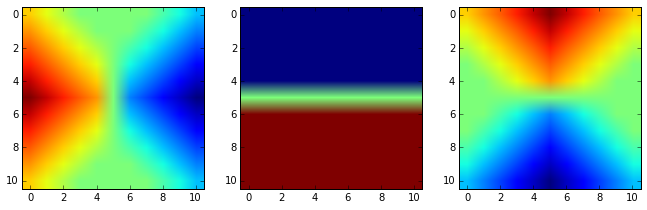
\includegraphics[width=0.3\textwidth]{./images/3filters.jpg}
	\caption{The three convolution kernels used for the architectures with three rows.}
	\label{fig:3filters}
\end{figure}

\begin{figure}[h!]
	\centering
	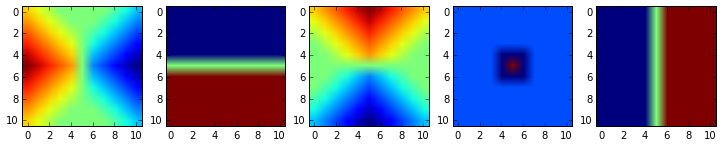
\includegraphics[width=0.5\textwidth]{./images/5filters.jpg}
	\caption{The five convolution kernels used for the architectures with five rows.}
	\label{fig:5filters}
\end{figure}

\begin{figure}[h!]
	\centering
	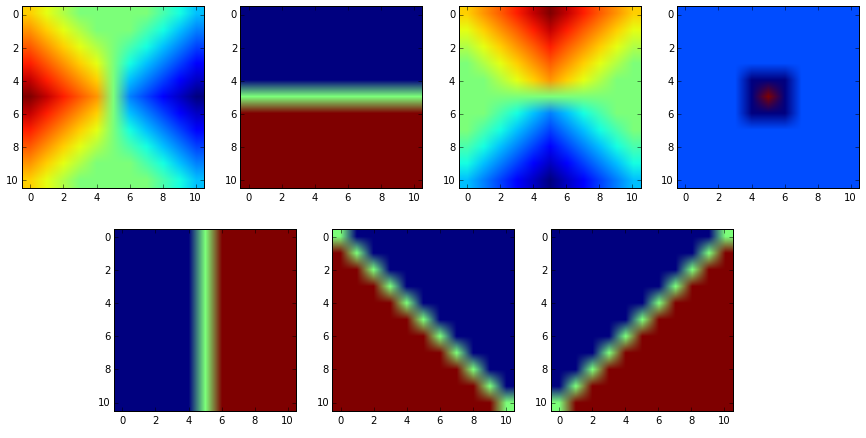
\includegraphics[width=0.4\textwidth]{./images/7filters.jpg}
	\caption{The seven convolution kernels used for the architectures with seven rows.}
	\label{fig:7filters}
\end{figure}

\end{appendices}






\end{document}



